
% Chapter 3 - Trend Analysis 
% --------------------------
% Jun 1, 2015


\chapter{Volume loss from Antarctic ice shelves is accelerating}

\noindent
This chapter, in full, is a reprint of:

\noindent
Paolo, F. S., H. A. Fricker, L. Padman, Volume loss from Antarctic ice shelves
is accelerating, {\it Science}, 348 (2015). doi:10.1126/science.aaa0940

\section*{}

\noindent
{\bf
The floating ice shelves surrounding the Antarctic Ice Sheet restrain the
groun\-ded ice-sheet flow. Thinning of an ice shelf reduces this effect, leading
to an increase in ice discharge to the ocean. Using 18 years of continuous
satellite radar altimeter observations, we have computed decadal-scale changes
in ice-shelf thickness around the Antarctic continent. Overall, average
ice-shelf volume change accelerated from negligible loss at 25 $\pm$ 64 cubic
kilometers per year for 1994--2003 to rapid loss of 310 $\pm$ 74 cubic
kilometers per year for 2003--2012. West Antarctic losses increased by
$\sim$70\% in the past decade, and earlier volume gain by East Antarctic ice
shelves ceased. In the Amundsen and Bellingshausen regions, some ice shelves
have lost up to 18\% of their thickness in less than two decades.
}

\section*{}

\noindent
\lettrine{T}{he Antarctic} Ice Sheet gains mass through snowfall and loses
mass at its margin through submarine melting and iceberg calving. These losses
occur primarily from ice shelves, the floating extensions of the ice sheet.
Antarctica's grounded-ice loss has increased over the past two decades
\parencite{Shepherd2012, Sutterley2014}, with the most rapid losses being along
the Amundsen Sea coast \parencite{Joughin2011} concurrent with substantial
thinning of adjoining ice helves \parencite{Shepherd2010, Pritchard2012} and
along the Antarctic Peninsula after ice-shelf disintegration events \parencite{
Scambos2004}. Ice shelves restrain ("buttress") the flow of the grounded ice
through drag forces at the icerock boundary, including lateral stresses at
sidewalls and basal stresses where the ice shelf rests on topographic highs
\parencite{Schoof2007, Goldberg2009}. Reductions in iceshelf thickness reduce
these stresses, leading to a speed-up of ice discharge. If the boundary between
the floating ice shelf and the grounded ice (the grounding line) is situated on
a retrograde bed (sloping downwards inland), this process leads to faster rates
of ice flow, with potential for a self-sustaining retreat \parencite{
Schoof2007, Favier2014, Joughin2014}.

Changes in ice-shelf thickness and extent have primarily been attributed to
varying atmospheric and oceanic conditions \parencite{Scambos2003a, Dutrieux2014}.
Observing iceshelf thickness variability can help identify the principal 
processes influencing how changing large-scale climate affects global sea level
through the effects of buttressing on the Antarctic Ice Sheet. The only
practical way to map and monitor ice-shelf thickness for this vast and remote
ice sheet at the known space and time scales of ice-shelf variability is with
satellite altimetry. Previous studies have reported trends based on simple line
fits to time series of ice-shelf thickness (or height) averaged over entire ice
shelves or broad regions \parencite{Shepherd2010, Zwally2005} or for short 
($\sim$5-year) time intervals \parencite{Pritchard2012, Rignot2013,Depoorter2013}.
Here, we present a record of ice-shelf thickness that is highly resolved in 
time ($\sim$3 months) and space ($\sim$30 km), using the longest available 
record from three consecutive overlapping satellite radar altimeter missions
(ERS-1, 1992--1996; ERS-2, 1995--2003; and Envisat, 2002--2012) spanning 18
years from 1994 to 2012.

Our technique for ice-shelf thickness change detection is based on crossover
analysis of satellite radar altimeter data, in which time-separated height 
estimates are differenced at orbit intersections \parencite{Zwally2005, 
Davis2004, Wingham2009}. To cross-calibrate measurements from the different 
satellite altimeters, we used the roughly 1-year overlap between consecutive
missions. The signal-to-noise ratio of altimeterderived height differences for
floating ice in hydrostatic equilibrium is roughly an order of magnitude 
smaller than over grounded ice, requiring additional data averaging to obtain
comparable statistical significance. We aggregated observations in time 
(3-month bins) and space ($\sim$30-km cells). Because the spatial distribution
of crossovers changes with time (due, for example, to nonexact repeat tracks
and nadir mispointing), we constructed several records at each cell location
and stacked them in order to produce a mean time series with reduced
statistical error\footnote{\label{SM}Materials and methods are available as 
supplementary materials on {\it Science} Online, and reproduced at the end of
the main text.}. We converted our height-change time series and rates to
thickness changes by assuming that observed losses occurred predominantly at
the density of solid ice (basal melting) \parencite{Shepherd2010,
Pritchard2012, Wingham2009}. This is further justified by the relative
insensitivity of radar measurements to fluctuations in surface mass 
balance\footnotemark[1]. For volume changes, we tracked the minimum (fixed) area of
each ice shelf\footnotemark[1]. We assessed uncertainties for all estimates using
the bootstrap approach (resampling with replacement of the residuals of the
fit) \parencite{Efron1993}, which allows estimation of formal confidence
intervals. All our uncertainties are stated at the 95\% confidence level 
[discussion of uncertainties are provided in \footnotemark[1] and the several
corrections applied are stated in \footnote{Corrections include lag of the
satellite's leading-edge tracker (retracking), surface scattering variations,
surface slope, dry atmospheric mass, water vapor, the ionosphere, solid Earth
tide, ocean tide and loading, atmospheric pressure, and regional sea-level
variation\footnotemark[1].}].

We estimated 18-year trends in ice-shelf thickness by fitting low-order 
polynomials (degree n $\leqslant$ 3) to the data using a combination of lasso
regularized-regression \parencite{Tibshirani1996} and cross-validation for
model-parameter selection (the shape of the fit is determined by the data).
This combined approach allowed us to minimize the effect of shortterm
variability on the 18-year trends. Relative to previous studies
\parencite{Shepherd2010, Pritchard2012, Zwally2005, Fricker2012}, we have
improved estimations by (i) using 18-year continuous records, (ii) implementing
a time series averaging scheme so as to enhance the signal-to-noise ratio, and
(iii) using a robust approach to trend extraction.

The 18-year average rate of thickness change varies spatially (Figure \ref{fig1ch3}).
On shorter time scales, trends are highly variable but spatially coherent
(Figure \ref{fig2ch3} and movie S1\footnote{include link to the movie.}). We divided
our data set into eight regions on the basis of spatial coherence of long-term
ice-shelf behavior and calculated time series of ice-shelf thickness change
(relative to series mean) for each region (Figure \ref{fig3ch3}). The largest regional
thickness losses were in the Amundsen and Bellingshausen seas, with average
(and maximum) thinning rates of 19.4 $\pm$ 1.9 (66.5 $\pm$ 9.0) m/decade and
7.4 $\pm$ 0.9 (64.4 $\pm$ 4.9) m/decade, respectively. These values correspond
to $\sim$8 and 5\% of thickness loss over the 18 years for the two regions,
respectively. These two regions account for less than 20\% of the total West
Antarctic ice-shelf area but, combined, contribute more than 85\% of the total
ice-shelf volume loss from West Antarctica. The area-averaged time records of
ice-shelf thickness and volume for the West and East Antarctic sectors 
(Figure \ref{fig1ch3}, bottom left), broad regions (Figure \ref{fig3ch3}), and single ice
shelves (Figure \ref{figs1ch3}) at 3-month time intervals show a wide range of
temporal responses with large interannual-to-decadal fluctuations, stressing
the importance of long records for determining the long-term state of the ice
shelves. Comparing our long records with simple linear trends obtained for the
periods of single satellite missions [such as the 5-year ICESat time span used
in \textcite{Pritchard2012}] shows that it is often not possible to capture the
persistent signals in the shorter records (Figure \ref{fig3ch3} and \ref{figs1ch3}).


\begin{figure}[!ht]
  \includegraphics[width=\textwidth]{../img/Fig1_dzdt_map_v10_all}
  \caption{{\bf Eighteen years of change in thickness and volume of Antarctic
  ice shelves.} Rates of thickness change (meters per decade) are colorcoded
  from $-$25 (thinning) to $+$10 (thickening). Circles represent percentage of
  thickness lost (red) or gained (blue) in 18 years. Only significant values at
  the 95\% confidence level are plotted (table \ref{tabs1ch3}). (Bottom left)
  Time series and polynomial fit of average volume change (cubic kilometers)
  from 1994 to 2012 for the West (in red) and East (in blue) Antarctic ice
  shelves. The black curve is the polynomial fit for All Antarctic ice shelves.
  We divided Antarctica into eight regions (Figure \ref{fig3ch3}), which are labeled
  and delimited by line segments in black. Ice-shelf perimeters are shown as a
  thin black line. The central circle demarcates the area not surveyed by the
  satellites (south of 81.5\degree S). Original data were interpolated for
  mapping purposes (percentage area surveyed of each ice shelf is provided in
  table \ref{tabs1ch3}). Background is the Landsat Image Mosaic of Antarctica
  (LIMA).}
  \label{fig1ch3}
\end{figure}


\begin{figure}[!ht]
  \includegraphics[width=\textwidth]{../img/Fig2_pannels_review_v4_rgb}
  \caption{{\bf Variability in the rate of Antarctic ice-shelf thickness change
  (meters per year).} Maps for (columns from left to right) Filchner-Ronne,
  Amundsen,and Ross ice shelves (locations in the bottom right corner) showing
  average rate of thickness change for (rows) four consecutive 4.5-year
  intervals (1994--1998.5, 1998.5--2003, 2003--2007.5, and 2007.5--2012).
  Shorter-term rates can be higher than those from an 18-year interval.
  Ice-shelf perimeters are thin black lines, and the thick gray line demarcates
  the limit of satellite observations.}
  \label{fig2ch3}
\end{figure}


\begin{SCfigure}[.6][!ht]
  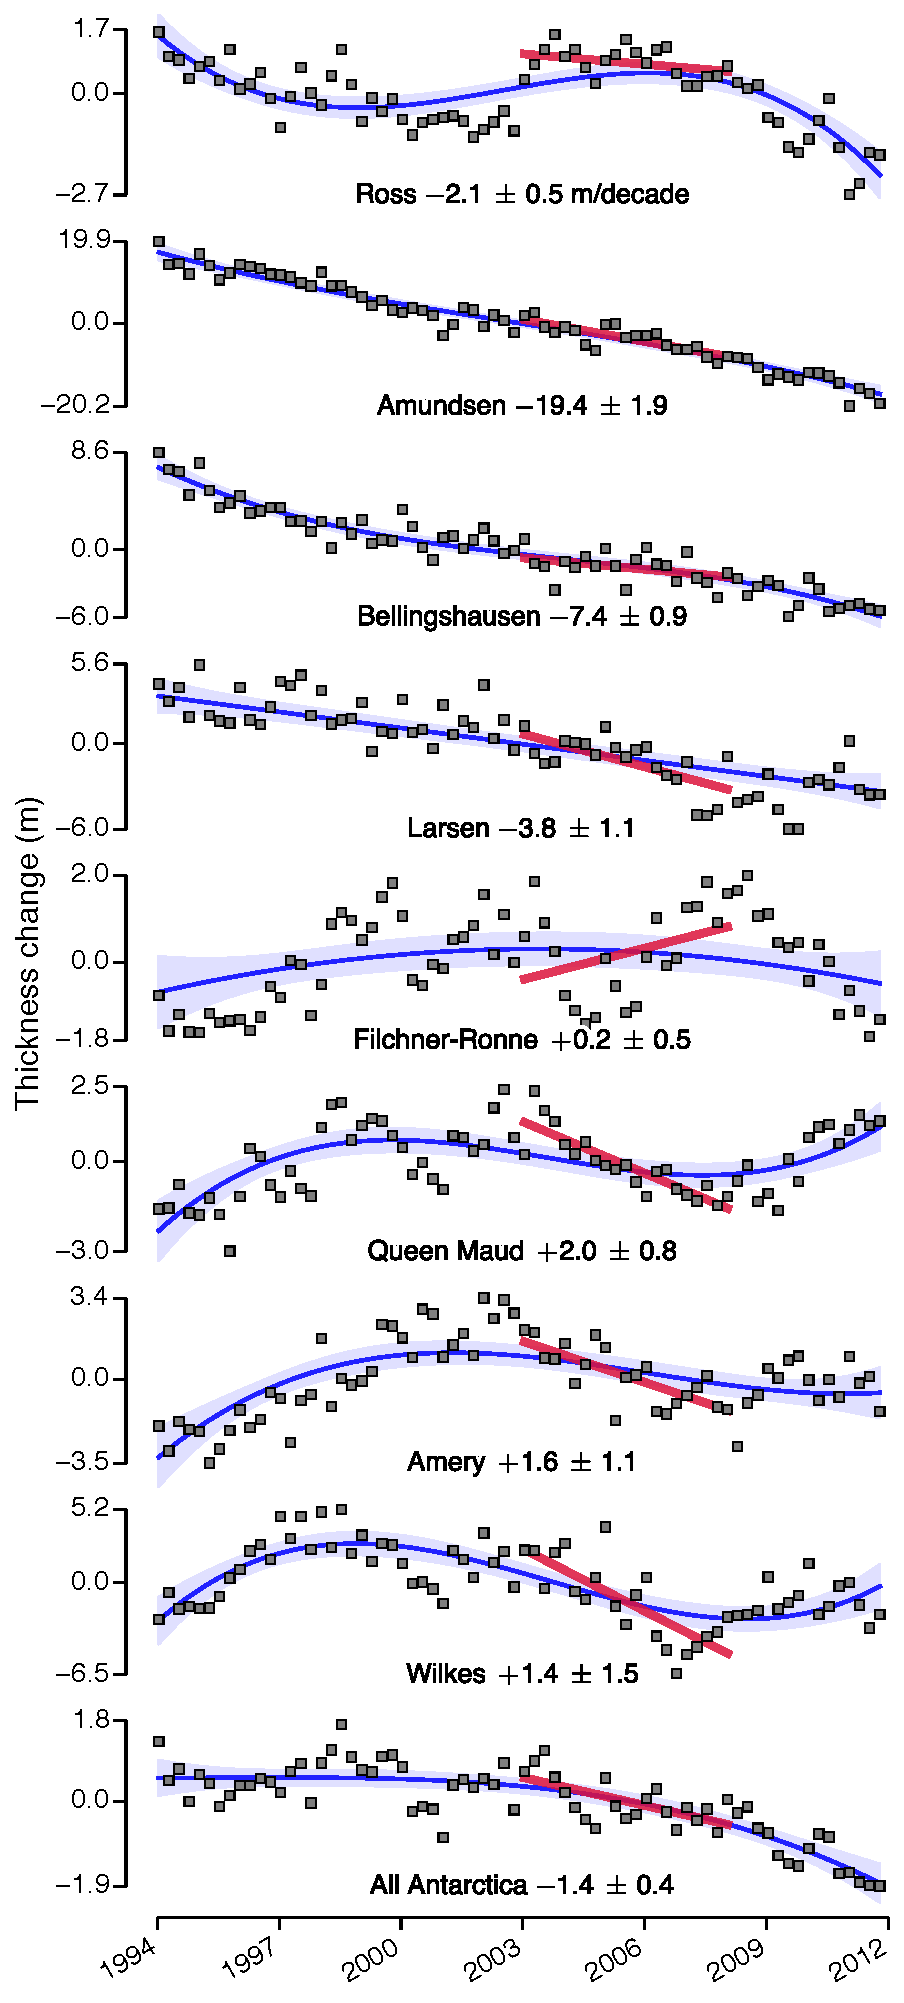
\includegraphics[width=.6\textwidth]{../img/Fig3_ts_regions_review_v6}
  \caption{{\bf Time series of cumulative thickness change relative to series
  mean for Antarctic ice-shelf regions (1994--2012).} Time series correspond to
  averages for all ice-shelf data within the Antarctic regions defined in
  Figure \ref{fig1ch3}. Dots represent average thickness change every 3 months. Error
  bars are small (in many cases, smaller than the symbols themselves, thus
  omitted from the plots), making the interannual fluctuation shown by the dots
  significant. The blue curve is the long-term trend from polynomial regression
  with the 95\% confidence band {\bf NOTE: Materials and methods are available as 
  supplementary materials on {\it Science} Online, and reproduced at the end of
  the main text.}. We converted our height-change time series and rates to, and
  the red line shows the regression line to the segment of our data set that
  overlaps with the period used for a prior ICESat-based analysis (2003--2008)
  \parencite{Pritchard2012}. Average rates (in meters per decade) are derived
  from the end points of the polynomial models.}
  \label{fig3ch3}
\end{SCfigure}


Ice-shelf average thinning rates from the 18-year polynomial fits in the
Amundsen Sea region (AS) range from 1.5 $\pm$ 0.9 m/decade for Abbot to 
31.1 $\pm$ 5.4 m/decade for Crosson, with local maximum thinning of 
66.5 $\pm$ 9.0 m/decade on Getz (Figure \ref{figs1ch3} and table
\ref{tabs1ch3}). Crosson and Getz have lost $\sim$18 and 6\% of their
thicknesses, respectively, over the 18-year period. If this thinning persists
for these two ice shelves, we can expect volume losses of $\sim$100 and 30\%,
respectively, in the next 100 years. Getz is the single largest contributor to
the overall volume loss of Antarctic ice shelves, with an average change of 
$-$54 $\pm$ 5 km$^3$/year, accounting for $\sim$30\% of the total volume loss
from theWest Antarctic ice shelves (table \ref{tabs1ch3}). We find the most
dramatic thickness reduction on Venable Ice Shelf in the Bellingshausen Sea
(BS), with an average (and maximum) thinning rate of 36.1 $\pm$ 4.4
(64.4 $\pm$ 4.9) m/decade, respectively (Figure \ref{figs1ch3} and table
\ref{tabs1ch3}). This ice shelf has lost 18\% of its thickness in 18 years,
which implies complete disappearance in 100 years.

For the ice shelves in the AS, observed rates
are highest near the deep grounding lines, with
lower rates found toward the shallower ice fronts
(Figure \ref{fig2ch3}, table \ref{tabs1ch3}, and movie \ref{movs1ch3}). This pattern is
consistent with enhanced melting underneath
the ice shelf forced by an increased flux of circumpolar
deep water (CDW) from across the continental
shelf and into the sub–ice-shelf cavity
\parencite{Dutrieux2014, Jacobs2011, Thoma2008}. The consequent loss of ice-shelf buttressing
from increased ocean-forced melting may
have driven the grounding lines inland \parencite{Rignot2014} to
a point on a retrograde bed slope at which the
marine ice-sheet instability mechanism can take
over the dynamics of ice export \parencite{Schoof2007, Weertman1974}. Hence,
observed ice-shelf thinning reflects both ocean-induced
basal melting and increased strain rates
resulting from faster flows. Our analysis shows
that thinning was already under way at a substantial
rate at the start of our record in 1994.

On the eastern side of the Antarctic Peninsula
[comprising Larsen B (Scar Inlet remnant), Larsen 
C, and Larsen D], the regional ice-shelf thinning
rate of 3.8 $\pm$ 1.1 m/decade (Figure \ref{fig3ch3}) is about half of
that on the western side (BS) (Figure \ref{fig1ch3}). The onset of
thinning for Larsen C has progressed southward
(Figure \ref{fig4ch3}), which is consistent with climate-driven
forcing discussed in earlier studies \parencite{Fricker2012, Cook2010}. The
highest thinning rates on Larsen C (with local
maximum thinning of 16.6 $\pm$ 8.1 m/decade) are
near Bawden Ice Rise (Figures \ref{fig1ch3} and \ref{fig4ch3}). Assuming
that half of this observed thinning is due to air
loss within the firn column, and considering
that the ice shelf is $\sim$40 m above flotation over
the ice rise \parencite{Holland2015}, we can expect Larsen C to fully
unground from this pinning point within the
next 100 years, with potential consequences on
the ice-shelf stability \parencite{Borstad2013}.


\begin{figure}[!ht]
  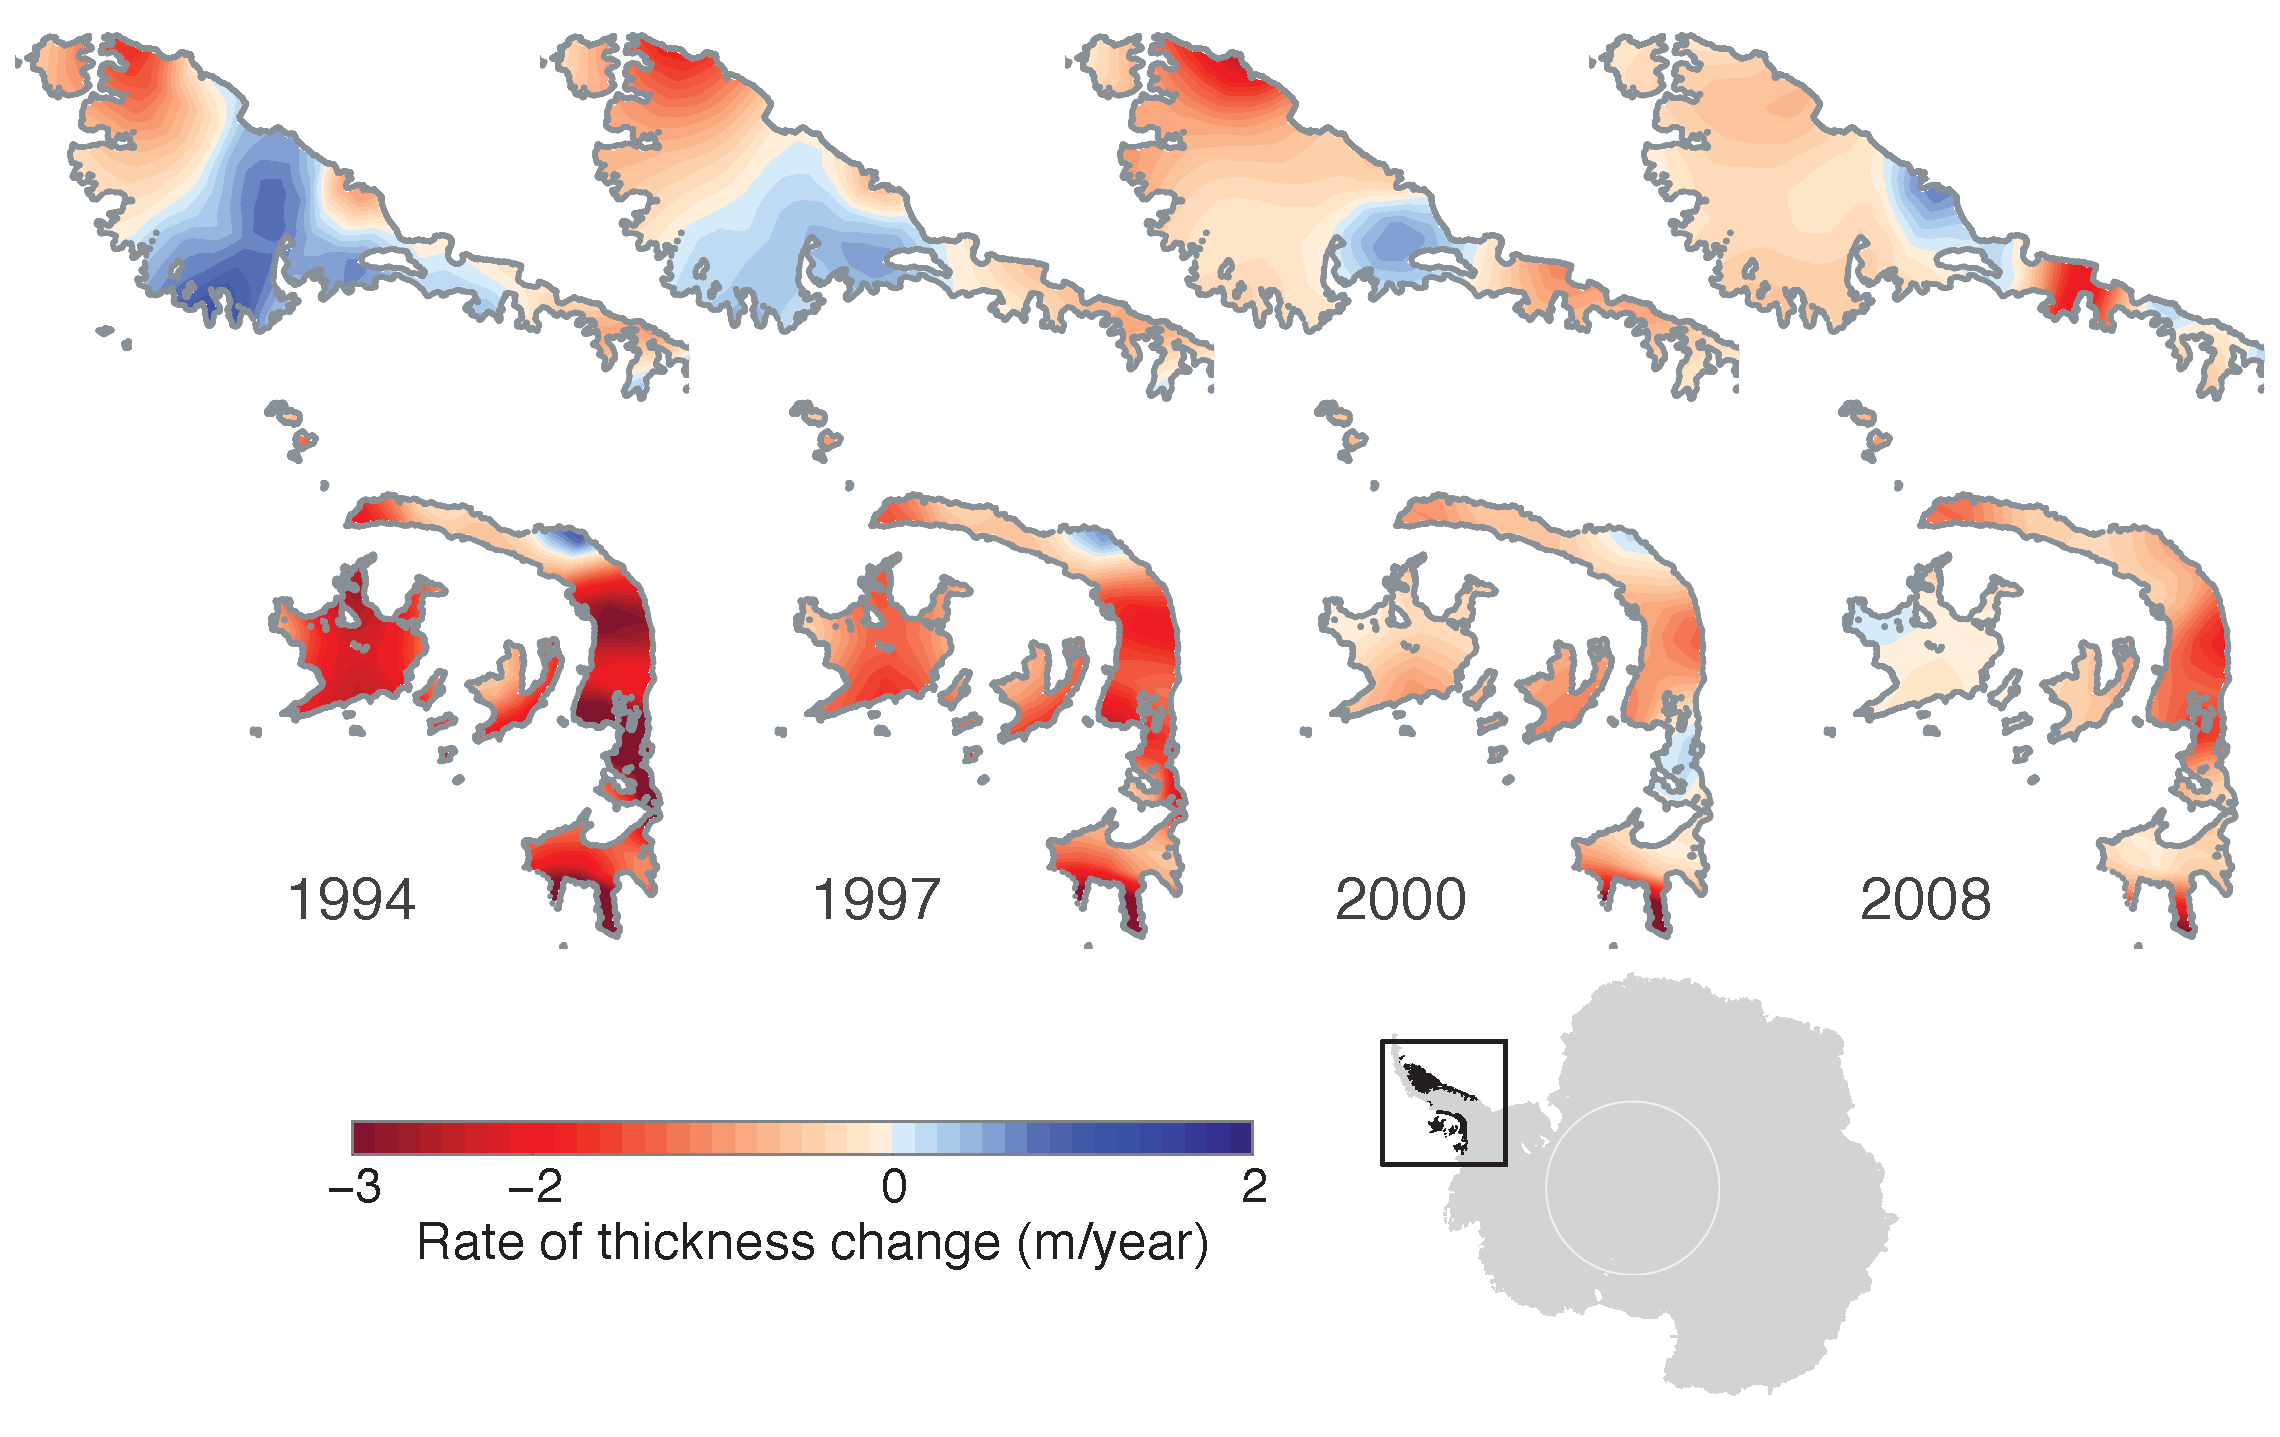
\includegraphics[width=\textwidth]{../img/Fig4_antpen_pannels_review_v5_cmyk.pdf}
  \caption{{\bf
  Evolution of the rate of thickness
  change in the Antarctic Peninsula.} Instantaneous
  rate-of-thickness change (meters per year) for
  four specific times (1994, 1997, 2000, and 2008)
  is calculated as the derivative of the polynomial fit
  to the thickness-change time series. The rate
  increases spatially with time from north to south
  in the Larsen Ice Shelf (movie \ref{movs1ch3}). The eastern
  (Weddell Sea) side of the Antarctic Peninsula (top)
  shows independent behavior from the western
  (Bellingshausen Sea) side (bottom).
  }
  \label{fig4ch3}
\end{figure}


The regional time-varying trends for the ice
shelves in the three East Antarctic regions (Queen
Maud, Amery, and Wilkes) are coherent (Figure \ref{fig3ch3}).
Ice shelves in the Wilkes region are challenging
for conventional radar altimeters because many
of them are small, contained in narrow embayments,
and have rough surfaces so that altimeter-derived
height changes do not necessarily reflect
thickness change accurately. Our estimate of overall
thickness change for the Wilkes ice shelves is
1.4 $\pm$ 1.5 m/decade, which is not significantly
different from zero. The Queen Maud region ice
shelves show an overall increase in thickness of
2.0 $\pm$ 0.8 m/decade.

Like the AS ice shelves, Totten and Moscow
University ice shelves in the Wilkes region buttress
a large marine-based section of the East
Antarctic ice sheet so that their stability is potentially
important to grounded-ice loss. Although
these ice shelves were previously reported as
thinning \parencite{Pritchard2012} on the basis of a straight-line fit to
a 5-year record from a satellite laser altimeter
(ICESat, 2003--2008), our results show that those
estimates are not representative of the longerterm
trends (Figure \ref{figs1bch3}). Our estimate of thickness
loss during 2003--2008 is similar to the ICESat-based
result, but the full 18-year period shows
thickness trends that are not significantly different
from zero (Figure \ref{figs2ch3}).

For most ice shelves, our estimates are significantly
different from previous results (Table \ref{tabs2ch3}).
Several factors contribute to this. (i) The areas of
ice shelves over which measurements are averaged
vary between studies, affecting estimates on
small ice shelves with large thickness-change
signals. (ii) Because of our grid resolution, ice
shelfmask, and limited data coverage, we cannot
sample near the grounding line of some ice shelves
(such as Pine Island or Dotson); in such cases,
our estimated changes are likely to represent a
lower bound (changes could be larger). (iii) Radar
altimeters are less sensitive than are laser altimeters
to variations in surface mass balance owing
to penetration of the radar signal into the firn
layer. (iv) Short records and previous trend-extraction
approaches could not capture and account
for fluctuations in the underlying trend (Figure \ref{figs3ch3}).
This is the dominant factor affecting comparisons
between our results and previous studies.

The total volume of East Antarctic ice shelves
increased during 1994--2003 by 148 $\pm$ 45 km$^3$/year,
followed by moderate loss (56 $\pm$ 37 km$^3$/year),
whereas West Antarctic ice shelves exhibited
persistent volume loss over the 18 years, with
marked acceleration after 2003 (Figure \ref{fig1ch3}). Before
and after 2003, this region lost volume by 144 $\pm$ 45 and 
242 $\pm$ 47 km$^3$/year, respectively, corresponding
to $\sim$70\% increase in the average loss
rate. The total circum-Antarctic ice-shelf volume
loss was negligible (25 $\pm$ 64 km$^3$/year) during
1994--2003 and then declined rapidly by 
310 $\pm$ 74 km$^3$/year after 2003. Overall, from 1994 to
2012 Antarctic ice-shelf volume changed on average
by $-$166 $\pm$ 48 km$^3$/year, with mean acceleration
of $-$31 $\pm$ 10 km$^3$/year$^2$ ($-$51 $\pm$ 33 km$^3$/year$^2$ for the
period 2003--2012).

We have shown that Antarctic ice-shelf volume
loss is accelerating. In the Amundsen Sea,
some ice shelves buttressing regions of grounded
ice that are prone to instability have experienced
sustained rapid thinning for almost two decades.
If the present climate forcing is sustained, we
expect a drastic reduction in volume of the rapidly
thinning ice shelves at decadal to century
time scales, resulting in grounding-line retreat
and potential ice-shelf collapse. Both of these processes
further accelerate the loss of buttressing,
with consequent increase of grounded-ice
discharge and sea-level rise. On smaller scales,
ice-shelf thickness variability is complex, demonstrating
that results from single satellite missions
with typical durations of a few years are
insufficient to draw conclusions about the long-term
response of ice shelves. Large changes occur
over a wide range of time scales, with rapid variations
of ice-shelf thickness suggesting that ice
shelves can respond quickly to changes in oceanic
and atmospheric conditions.

\section*{Materials and Methods}

\subsection*{Antarctic ice-shelf mask}

To precisely define the ice-shelf boundaries ({\it e.g.}, grounding lines, ice
fronts) we used a 1-km-resolution Antarctic mask \parencite{Depoorter2013},
constructed using a composite of InSAR \parencite{Rignot2011}, ICESat 
\parencite{Fricker2006, Brunt2010}, MOA \parencite{Scambos2007} and ASAID
\parencite{Bindschadler2011} products.

\subsection*{Raw radar altimeter data editing}

Our satellite radar altimeter data are from NASA/GSFC's Version 4 Level 2 Ice
Data Records\footnote{\tt http://icesat4.gsfc.nasa.gov/radar\_data/data\_products.php}.
We rejected altimeter height estimates in the following cases: i) The return
altimeter waveform had no leading edge, meaning that the part of the return 
corresponding to the surface was not captured; ii) The waveform had a shape 
indicating specular reflection, which could indicate the presence of ponded 
surface water (35); iii) One or more geophysical corrections were missing; 
iv) The point was located within 3 km of any ice-shelf boundary (grounding 
line or ice front); this removed across-boundary measurements and minimized 
the impact of changes in ice-shelf perimeter.

\subsection*{Altimeter data corrections}

All satellite radar altimeter data were retracked with the 5-parameter 
$\beta$-retracker algorithm \parencite{Brenner1983}. We corrected for surface
scattering variations for each satellite mission independently, similar to 
\textcite{Zwally2005, Davis2004}, and \textcite{Wingham2009}. We found that
over the ice shelves those methods provided more consistent results ({\it i.e.}, 
similar performance over a wide range of surface conditions) than accounting 
for short-time variability of surface properties as done by 
\textcite{Khvorostovsky2012}. We corrected for tides using the Circum-Antarctic
Tidal Simulation CATS2008a (updated from \textcite{Padman2002}), and load tide
based on the TPXO7.2 ocean tide model \parencite{Egbert2002}. We corrected for
trends in atmospheric pressure (inverse barometer) using values from the 
ERA-Interim (global atmospheric reanalysis) to estimate $dP_{\text{air}}/dt$
(mbar/year) for 1994--2012 \parencite{Padman2003}. We corrected for regional
sea-level trends using the AVISO SSALTO\/DUACS multi-mission altimeter product
\parencite{LeTraon1998}, propagating and smoothing values for the unsurveyed
regions underneath ice shelves and persistent sea ice. Many of these
corrections are small compared to the magnitude of long-term thickness-change
signals.

Radar-altimeter observations are relatively insensitive to fluctuations in the
firn column due to radar signal penetration into the firn layer (unlike laser
pulses from laser altimeters that reflect from the surface). We did not 
attempt to make a firn correction based on RACMO \parencite{vanMeijgaard2008}
as has been adopted by some other researchers ({\it e.g.}, \textcite{Pritchard2012}),
as we found no significant correlation between the modeled firn-height trends
and our observed height-change trends. Furthermore, we know from work on the
Amery Ice Shelf \parencite{Phillips1999} that the radar extinction coefficient
derived from the return waveform (which is inversely proportional to
penetration depth) is higher on the ice shelf than it is on the drier parts of
the ice-sheet interior ({\it i.e.}, penetration is lower for the ice shelves than
for the ice-sheet interior). Additionally, in the vast majority of grid cells,
densification of the surface (a "competing" effect with penetration bias, {\it i.e.},
opposite sign) is by far the dominant effect, which we minimized by performing
a backscatter correction.

In summary, our estimates of time-dependent ice-shelf height account for the
lag of the satellite's leading-edge tracker, surface scattering variation,
surface slope, dry atmospheric mass, water vapor, the ionosphere, solid Earth
tide, ocean tide and loading, atmospheric pressure and regional sea-level
variation.

\subsection*{Derivation of height-change time series}

To estimate change in ice-shelf height at each location, we processed all
satellite radar altimeter data using crossover analysis where time-separated
height estimates are differenced at satellite orbit intersections 
\parencite{Zwally2005, Davis2004, Wingham2009}. We only used height differences
derived from the same mode of altimeter operation, {\it i.e.}, ocean-ocean or ice-ice
(ERS-1 and 2) and fine-fine (Envisat). We excluded any absolute height
difference greater than 15 m and applied a 3-sigma filtering.

To enhance the signal-to-noise ratio we performed two key averaging procedures
to construct our time series of height differences. i) Averaging in time and
space: we averaged the crossovers derived from differencing pairs of height
measurements taken from separate three-month bins and spatial cells of
0.75\degree $\times$ 0.25\degree in longitude and latitude, respectively 
($\sim$27 $\times$ 27 km at 71\degree S); ii) Averaging time series: we
extended the methods of \textcite{Li2006} and \textcite{Khvorostovsky2012},
where (in the previous step) all possible combinations between different
height sets at each cell location are differenced to form several time series
referenced to different epochs. This two-sided data matrix (one time series
per row) is then referenced to a common time and weight-averaged by number of
observations to produce a mean time series per cell, with reduced statistical
error. We estimated average height-change per cell as

\begin{equation}
  \overbar{\Delta h}(\mathbf{x}, t_i, t_j) = \frac{1}{n_\text{ad} + n_\text{da}} 
  \left\{
  n_\text{ad} \, \text{Md}\!\left[ \Delta h_\text{ad}(t_i, t_j) \right] +
  n_\text{da} \, \text{Md}\!\left[ \Delta h_\text{da}(t_i, t_j) \right]
  \right\}
\end{equation}

where $\overbar{\Delta h}$ is the mean height-change value between times $t_i$
and $t_j$, $\Delta h_\text{ad}$ and $\Delta h_\text{da}$ are height changes
formed by differencing ascending-descending and descending-ascending satellite
ground tracks, respectively, $n_\text{ad}$ and $n_\text{da}$ are the number of
crossovers of each type, and $\text{Md}[\,\,]$ is the median operator. The
(weighted) average between ascending/descending and descending/ascending
crossovers is necessary to remove any time-invariant biases, such as those
introduced by the combination of satellite orientation, antenna polarization
and ice surface anisotropy.

In the mean time series on each grid cell we removed step changes greater than
3 m ({\it e.g.}, resulting from anomalous backscatter), and also removed any peak
greater than 3 standard deviations from the polynomial trend (see below). We
rejected any time series with data points spanning less than 70\% of the
18-year time interval, or showing evidence (to the eye) of poor-quality data.

\subsection*{Estimating trends in ice-shelf height}

To estimate acceleration terms present within the underlying trends of the
height data, we fitted polynomial models (using penalized least squares, see
below) to the height-change time series allowing for the degree to vary from
$m = 0$ to 3, as

\begin{equation}
  \hat h(\tau) = \sum^3_{m=3} \beta_m \, \tau^m + \varepsilon
\end{equation}

where $\hat{h}(\tau)$ is the polynomial model, $\tau = t - 1994$, $\beta_m$
are the coefficients of the polynomial and $\varepsilon$ is the error term. We
then calculated average and instantaneous rates of change as the slope of the
secant and tangent lines, respectively, to the fitted polynomial (by finite
difference approximation). The average rate of height change is then given by

\begin{equation}
  \frac{\Delta \hat h}{\Delta \tau} = \frac{\hat h(\tau_j) - \hat h(\tau_i)}
  {\tau_j - \tau_i} + \dot p + \dot \eta
\end{equation}

where $\Delta \hat h / \Delta \tau$ is the rate of change between $\tau_i$ and
$\tau_j$, $\dot p$ is regional atmospheric-pressure trend (inverse barometer
effect), and $\dot \eta$ is regional sea-level trend. In practice, the higher
the complexity of the model, the better the fit and the worse the
generalization. To mitigate this, we chose to use the lasso approach
\parencite{Tibshirani1996} and a 10-fold cross-validation for regularized
regression and model-parameter selection, respectively. In some cases the more
robust polynomial-derived trends show substantial differences with respect to
trends derived from the ordinary straight-line fit (Figure \ref{figs4ch3}).

\subsection*{Estimating thickness and volume changes from height time series}

We converted our height-change time series and rates to thickness changes
assuming that (i) the ice shelf is in hydrostatic equilibrium and (ii)
observed changes occur at the density of solid ice ({\it e.g.}, basal melting;
\parencite{Shepherd2010, Pritchard2012, Wingham2009}. The latter assumption is
justified since, as discussed above, radar-altimeter measurements are
relatively insensitive to changes in surface mass balance. We used an ice
density of 917 kg/m$^3$ and ocean water density of 1028 kg/m$^3$.

To map the spatial patterns of thickness changes, we fitted polynomials to the
thickness-change time series for each grid cell and derived averaged rates as
described above. We then smoothed and interpolated the rate-of-change spatial
field using a Gaussian kernel with sigma equal to the grid-cell size. To
estimate full-ice-shelf and regional mean values we integrated the individual
time series, limited to the surveyed area only and weighted by grid-cell area
({\it i.e.}, ice-shelf area within each grid cell). The surveyed area is the fixed
area of cells covered by the satellites' orbits for which data are available
throughout 1994--2012, therefore excluding ice shelves south of 81.5\degree S
and regions of advancing and retreating ice fronts and grounding lines.
Overall, we were able to sample about 86\% of the ice-shelf area covered by
the ERS/Envisat orbit. Our area-average thickness-change time series are then

\begin{equation}
  H(\tau) = s \sum_k w_k \, h_k(\tau)
\end{equation}

where $H(\tau)$ is mean time series of thickness change,
$s = \rho_{\text{oce}} \, (\rho_{\text{oce}} - \rho_{\text{ice}})^{-1}$ is the
height-to-thickness scaling factor, $w$ are the weights for each cell $k$
in the area-weighted average, and $h(\tau)$ is the observed height-change time
series for each grid cell. To estimate the associated total ice-volume change
for each ice shelf, we multiplied the derived changes (from the polynomial
fits) on the surveyed area of each ice shelf by the full areas estimated
using the 1-km-resolution ice-shelf mask, as

\begin{equation}
  \frac{\Delta V}{\Delta \tau} = A \, s \, \frac{\Delta \hat h}{\Delta \tau}
\end{equation}

where $A$ is total ice-shelf/region area.

The extreme case for temporal changes in ice-shelf area is the addition of
$\sim$600 km$^2$ to the area of the Crosson and Dotson ice shelves due to
grounding-line retreat during the period of 1992--2012 \parencite{Rignot2014},
corresponding roughly to 7\% area increase. This area, which is excluded by
our analysis, is small compared to the area that we cannot survey due to other
constraints such as missing data, narrow embayments, rough topography,
proximity to ice-shelf margins, and grid resolution. There are several ice
shelves with more than 10\% area unsurveyed (see Table \ref{tabs1ch3}). The
error is also small relative to the height-to-volume conversion uncertainty
due to inability to partition volume loss between basal melt, ice divergence
and surface firn state. Uncertainties in the rate of thickness/volume change
for the surveyed minimum ice-shelf area are significantly larger than any
potential ice-shelf volume change by a retreating grounding line.

For calculating fractional change in ice-shelf volume we estimated the average
thickness of each ice shelf using the \emph{Bedmap2} dataset
\parencite{Fretwell2013}. To estimate average acceleration we calculated the
average rate of change (slope of the secant line) of the derivative of the
fitted polynomial.

\subsection*{Estimation of uncertainties}

Our averaging procedure facilitates the formal derivation of statistical error
for individual average-height values on every time series. Two factors
contribute to lower the uncertainty in our estimates: i) the large number of
crossovers that contribute to the final estimate per location per time step
(typically 10--150); and ii) the long records (18 years), which makes the
derivation of long-term slopes robust to high-frequency fluctuations ({\it e.g.},
seasonality).

Our uncertainties are meant to reflect (i) the sampling error ({\it i.e.}, amount of
information available), and (ii) the relative variability in location. Hence,
we derived the time-series error bars as

\begin{equation}
  \delta h(\mathbf x, \tau) = \sqrt{\text{SE}[\Delta h(\mathbf x, \tau)]^2 + 
  \text{SE}[h(\mathbf x)_\text{cor} - h(\mathbf x)_\text{unc}]^2}
\end{equation}

where $\text{SE}[\,\,]$ is the standard error,
$\overbar{\Delta h}(\mathbf x,\tau)$ represents all height changes at time
$\tau$ and grid-cell location $\mathbf x$, and $h(\mathbf x)$ is the mean time
series for each grid cell, backscatter corrected $(\text{cor})$ and
uncorrected $(\text{unc})$. The first term on the right hand side represents
the noise at the grid-cell level. The second term assesses the magnitude of
the backscatter-to-height correlation; that is, we assume that the true height
lies between the uncorrected and backscatter-corrected values. Notice that the
first term is the standard error propagated in the time series averaging
process, so that both terms refer to the mean time series.

For the fitted trends we estimated the uncertainties based on the variance of
the residuals, which are generally higher than the uncertainty derived from
the individual data points. This is because the spread of the residuals arises
from true natural variability in addition to observational uncertainty
(individual error bars). Furthermore, the spread of the residuals contain
valuable information on whether the fitted trend is a good statistical model
for the data. We computed the residuals as

\begin{equation}
  \varepsilon = h - \hat h
\end{equation}

where $\varepsilon$ are the residuals, $h$ is the observed time series of
height changes and $\hat h$ is the polynomial fit. We then used the bootstrap
approach to randomly subsample with replacement the residuals of the polynomial
fit \parencite{Efron1993}. That is, every subsample of the residuals contains
original samples that can appear multiple times, so that the subsamples have
the same number of observations as the original set, but with less information
about the noise (with respect to the fit) in the data. We then added back each
resampled residual to the original fitted model to construct the bootstrap
samples, {\it i.e.}

\begin{equation}
  h^* = \hat h + \varepsilon^* 
\end{equation}

where $h^*$ is the bootstrap time series and $\varepsilon^*$ are the resampled
residuals. To each bootstrap time series we then refitted the polynomial model
and calculated the following: average rate of change, the derivative of the
polynomial and the average rate of change of the derivative (average
acceleration). By doing this repeatedly, we constructed an empirical
distribution for each parameter of interest. From this distribution we then
estimated formal confidence intervals and standard errors. We constructed 1000
bootstrap samples for each individual ice-shelf time series, and 500 for each
grid-cell time series (a total of 1,330,000 sets of calculations).

There is also a systematic component to the uncertainty in the estimated
ice-shelf height rates, which comes from the regional sea-level change. The
error in the rate of change of ice-surface height has an order of magnitude of
millimeters-to-tens-of-centimeters per year, while the error in the regional
sea-level trend has an order of magnitude of a millimeter per year. The
uncertainty in the ice-shelf height rate is then given by

\begin{equation}
  \delta \dot{\hat h} = \sqrt{(\delta \dot{\hat h}^*)^2 + (\delta \dot \eta)^2}
\end{equation}

where $\delta \dot{\hat h}^*$ is the uncertainty in the rate of height change
at the 95\% confidence level from the bootstrap distribution, and
$\delta \dot \eta$ is the uncertainty in regional sea-level trend
\parencite{LeTraon1998}. For thickness and volume we scaled the uncertainties
in height by the height-thickness conversion factor and the full-ice-shelf
area, respectively.

Estimating uncertainties using bootstrapping (top-down approach) has the
advantage of not relying on the assumption that characteristics of the noise
are known ({\it e.g.}, normally distributed), or requiring that the relationships
between the different sources of error are specified since an algebraic
solution of error propagation (bottom-up approach) is not required.

\subsection*{Limitations of our study}

During the observation period, some ice shelves experienced significant
grounding-line retreat \parencite{Rignot2014}, meaning that the ice shelf
increased in area. This ice-shelf migration could impact the average value of
volume loss if the new ice-shelf thickness is taken into account, although
these area changes are small relative to the total ice-shelf area (less than
7\%). Since our objective is to map and quantify the varying impacts of the
ocean and atmosphere to ice loss around the Antarctic ice shelves, we use a
fixed area approach ({\it i.e.}, Eulerian reference frame).

We are unable to sample near the ice-shelf grounding line. This data loss is
most severe for small ice shelves that have large melt rates in the grounding
zone ({\it e.g.}, Pine Island and Dotson). This limitation is mainly due to: i) our
grid-cell size (which is limited by the spatial distribution of the satellite
ground-track crossing points) and good-quality data availability near boundary
transitions. This imposes a limitation on sampling the grounding lines of small
and narrow ice shelves; (ii) our 3-km buffer for ice-shelf boundaries. Although
this removes observations right at the grounding line, it avoids biasing
ice-shelf estimates with grounded-ice signal (an order of magnitude larger)
from the locations where grounded-ice changes are most accentuated. As a
result, our estimates for small and rapidly changing ice shelves can be
regarded as a lower bound, in particular those experiencing increased basal
melting conditions where large changes occur near the grounding line, {\it e.g.},
Pine Island. This means that the ice-shelf loss could be even higher, which
should be considered when comparing estimates from different approaches.
